\chapter{Ergebnisse}

Die Evaluation wurde primär durch ausprobieren getestet. 
Das Notebook Visualize.ipynb enthält Funktionen um jede der Varianten zu visualisieren.

\section{YOLOv5}
YOLOv5 ist das Modell, welches in diesem Projekt am wenigsten optimiert wurde.
Dies lag an der hohen Trainingszeit, durch die hohe Auslastung des Filtersystems.
Es wurde ein YOLOv5s Modell (relativ kleines Modell) über 2 Epochen mit einigen Frozen Layern des Backbones trainiert.
Leider sind die Resultate von diesem nicht zu gebrauchen.
Es werden anstatt die selbst definierten Labels immer noch Objekte der Kategorie 'Person' erkannt, was vermutlich durch entsteht, dass es sich um ein vortrainierte Modell handelt.
Im weiteren Verlauf wurde deshalb FasterRCNN anstatt YOLO genutzt.

\section{FasterRCNN + Keypoint Head}
\begin{figure}[!htb]
    \centering
    \fbox{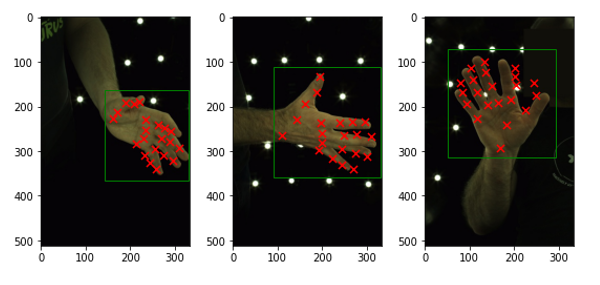
\includegraphics[width=15.5cm]{abbildungen/fasterrcnn_single_hand.PNG}}
    \caption{FasterRCNN+Keypoint Head, einzelne Hand}
    \label{fig:fasterrcnn_single}
\end{figure} 
Durch eine Aneinanderreihung des FasterRCNN Modells und der beiden Custom Keypoint Detection Heads, erhält man die beschriebene Architektur aus Kapitel \ref{ch:methods} (Abbildung \ref{fig:arch}).
Dabei detektiert FasterRCNN die Bounding Box der Hände sowie ob es sich dabei um einzelne oder interagierende Hände handelt.
Nachdem der Bildausschnitt innerhalb der Box ausgeschnitten wurde, wird dieses an entsprechendes Modell weitergegeben.
Die Keypoint-Predictions müssen jedoch vor der Visualisierung transformiert werden, da diese in einem Wertebereich zwischen 0 und 1 liegen.\\
Abbildung \ref{fig:fasterrcnn_single} zeigt einige gute Beispiele für die Erkennung einzelner Hände.
Die Keypoints sind relativ nah an den tatsächlichen Keypoints (Gelenken), jedoch oftmals einige Pixel versetzt.
Leider ist nicht jedes Ergebnis so gut, wie bei den dargestellten Beispielen.
Bei einigen Bildern sind die Keypoints geclustert in einer Ecke.
Jedoch ist der Ansatz vielversprechend und könnte durch zusätzliche Optimierungen, wie bspw Training mit mehreren Epochen, verbessert werden.\\

Anders sieht es jedoch bei interagierenden Händen aus,dort sind die Ergebnisse deutlich schlechter.
Wie in Abbildung \ref{fig:fasterrcnn_interagierend} sichtbar, sind die Keypoints oftmals geclustert.
Manchmal sind einige Keypoints auch in der oberen linken Ecke. 
Dies liegt daran, dass bei einigen Labels eine der beiden Hände fehlt, und alle Keypoints deshalb die Koordinaten (0,0) besitzen.
Durch mehrere und größere Schichten könnten sich die Ergebnisse verbessern.
Eine andere Alternative wäre es, zusätzlich noch Convolution Layers zu nutzen, welche die Keypoints als Heatmap lokalisieren, ähnlich wie bei KeypointRCNN.\\
\begin{figure}[!htb]
    \centering
    \fbox{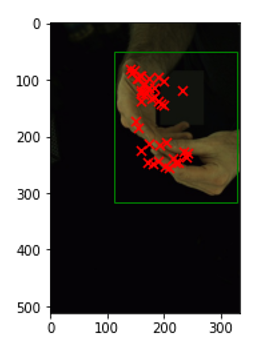
\includegraphics[width=5cm]{abbildungen/fasterrcnn_interacting.PNG}}
    \caption{FasterRCNN+Keypoint Head, interagierende Hände}
    \label{fig:fasterrcnn_interagierend}
\end{figure}


\section{KeypointRCNN}

Die besten Ergebnisse liefert KeypointRCNN. 
Da dieses Modell immer die gleiche Anzahl an Keypoints vorhersagt, wurde die Anzahl auf 42, 21 Keypoints pro Hand, gesetzt.
Abbildung \ref{fig:keypointrcnn_interagierend} zeigt einige Beispiele von interagierenden Händen.
Die Keypoints liegen sehr genau auf den Gelenken, welche durch diese kodiert werden.
Sogar wenn eine Hand die andere verdeckt (sichtbar in der Visualisierung rechts), werden die Keypoints der zweiten Hand korrekt dargestellt.\\
\begin{figure}[!htb]
    \centering
    \fbox{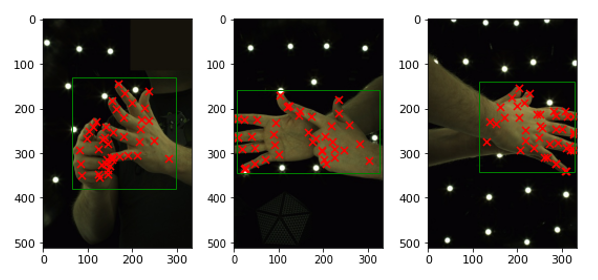
\includegraphics[width=15.5cm]{abbildungen/keypointrcnn_interacting.PNG}}
    \caption{KeypointRCNN, interagierende Hände}
    \label{fig:keypointrcnn_interagierend}
\end{figure} 
Sofern nur eine Hand im Bild ist, werden die Keypoints in der Regel aufeinander predicted, wie es Abbildung \ref{fig:keypointrcnn_single}. 
Dadurch sind es quasi 2 Keypoints pro Gelenk. 
In einem Post-Processing Schritt könnte man dies bei Bedarf raus filtern.
\begin{figure}[!htb]
    \centering
    \fbox{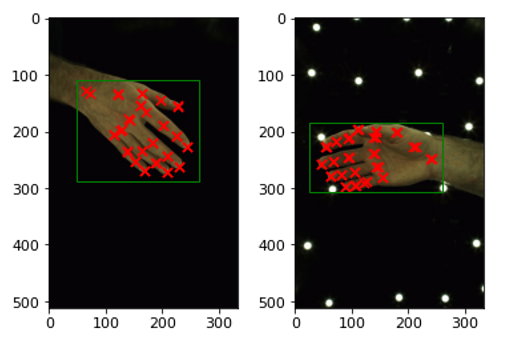
\includegraphics[width=10cm]{abbildungen/keypointrcnn_single.PNG}}
    \caption{KeypointRCNN, einzelne Hand}
    \label{fig:keypointrcnn_single}
\end{figure} 
